\documentclass[margin=5mm]{article}
\usepackage{tikz}
\usepackage{parskip}
\usepackage{listings}
\usepackage{color}
\usepackage{amsmath}


\usepackage[utf8]{inputenc}
\usepackage[english]{babel}
\usepackage{hyperref}
\usepackage{appendix}
\hypersetup{
    colorlinks=true,
    linkcolor=blue,
    filecolor=magenta,      
    urlcolor=cyan,
}
 
\urlstyle{same}

\usetikzlibrary{matrix,calc}
\definecolor{dkgreen}{rgb}{0,0.6,0}
\definecolor{gray}{rgb}{0.5,0.5,0.5}
\definecolor{mauve}{rgb}{0.58,0,0.82}

\lstset{frame=tb,
  aboveskip=3mm,
  belowskip=3mm,
  showstringspaces=false,
  columns=flexible,
  basicstyle={\small\ttfamily},
  numbers=none,
  numberstyle=\tiny\color{gray},
  keywordstyle=\color{blue},
  commentstyle=\color{dkgreen},
  stringstyle=\color{mauve},
  breaklines=true,
  breakatwhitespace=true,
  tabsize=3
}

\title{The SEND Model}
\author{
    Mastodon C}
\date{\today}



\begin{document}
\maketitle

\tableofcontents
\section{SEND Population Model}

\subsection{Model Entities, Terminology, and Prediction}\label{summary}
From Simulation, Modeling and Analysis \cite[ch.~1,p.~3]{sma4}:

\begin{quote}
``The state of a system is defined to be the collection of variables
necessary to describe a system at a particular point in time, relative
to the objective of a study.''
\end{quote}

and

\begin{quote}
``A system is defined to be the collection of entities that act and
interact towards the accomplishment of some goal.''
\end{quote}

In the SEND Model the collection of entities that make up the system
are drawn from $S \times N \times AY$ where

$S = \{MMSIB, ISS, ISSR, \dots, MU\}$

$N = \{CL, \dots, NONSEND\}$

$AY = \{4, \dots, 24\}$

For a given local authority, $S$ represents the set of valid types of
school setting, $N$ represents the set of valid need types, and $AY$
is the set of allowable academic years in SEND.  In the case of our
model, an `entity' is a unique combination of setting/need/academic
year, and we are interested in knowing the `population' (number of
pupils) in that entity.

Academic Year is a somewhat overloaded term: however in this document,
for historic reasons, it is used to represent the National Curriculum
Year.

Each entity has a single state variable $t$ which represents
its total population - it will always be a non-negative integer.

The points in time for which we can examine an entity's state is per
calendar year.

The SEND simulation predicts the population of each of the system
entities from one calendar year to the next using the following:

\begin{itemize}
\item The current entities population.
\item Predicted future pupil populations at an Academic Year level (not at
  an entity level i.e., ONS data).
\item Probability distributions generated from historical data.
\end{itemize}

One further note on the terminology; `state' is a contextual word
whose scope changes to encompass our current level of thinking e.g.,
the `system state' is the collection of all entities with their
particular state variables at a point in time.  Whereas an entity's
`state' is the collection of its state variables only - or in our
model's case, as there is only one state variable, it's simply the
population of the entity.  Further, `state' has been used in the
code-base to represent a need-setting pair.  In this document we will
endeavour to always qualify `state' for clarity.

\subsection{Visualising and Initialising System State}
By visualising the mathematical structures that govern system state we
can gain an intuitive understanding of how the model works.  In
Fig.\ref{state}, $t_{s_x,n_y,ay_z}$ represents the total population of
some setting $s_x$, need $n_y$ and academic year $ay_z$.  Where $x$,
$y$, $z$ are any integer index into the respective ordered sets: $S$,
$N$, $AY$.

\begin{figure}[h!]
  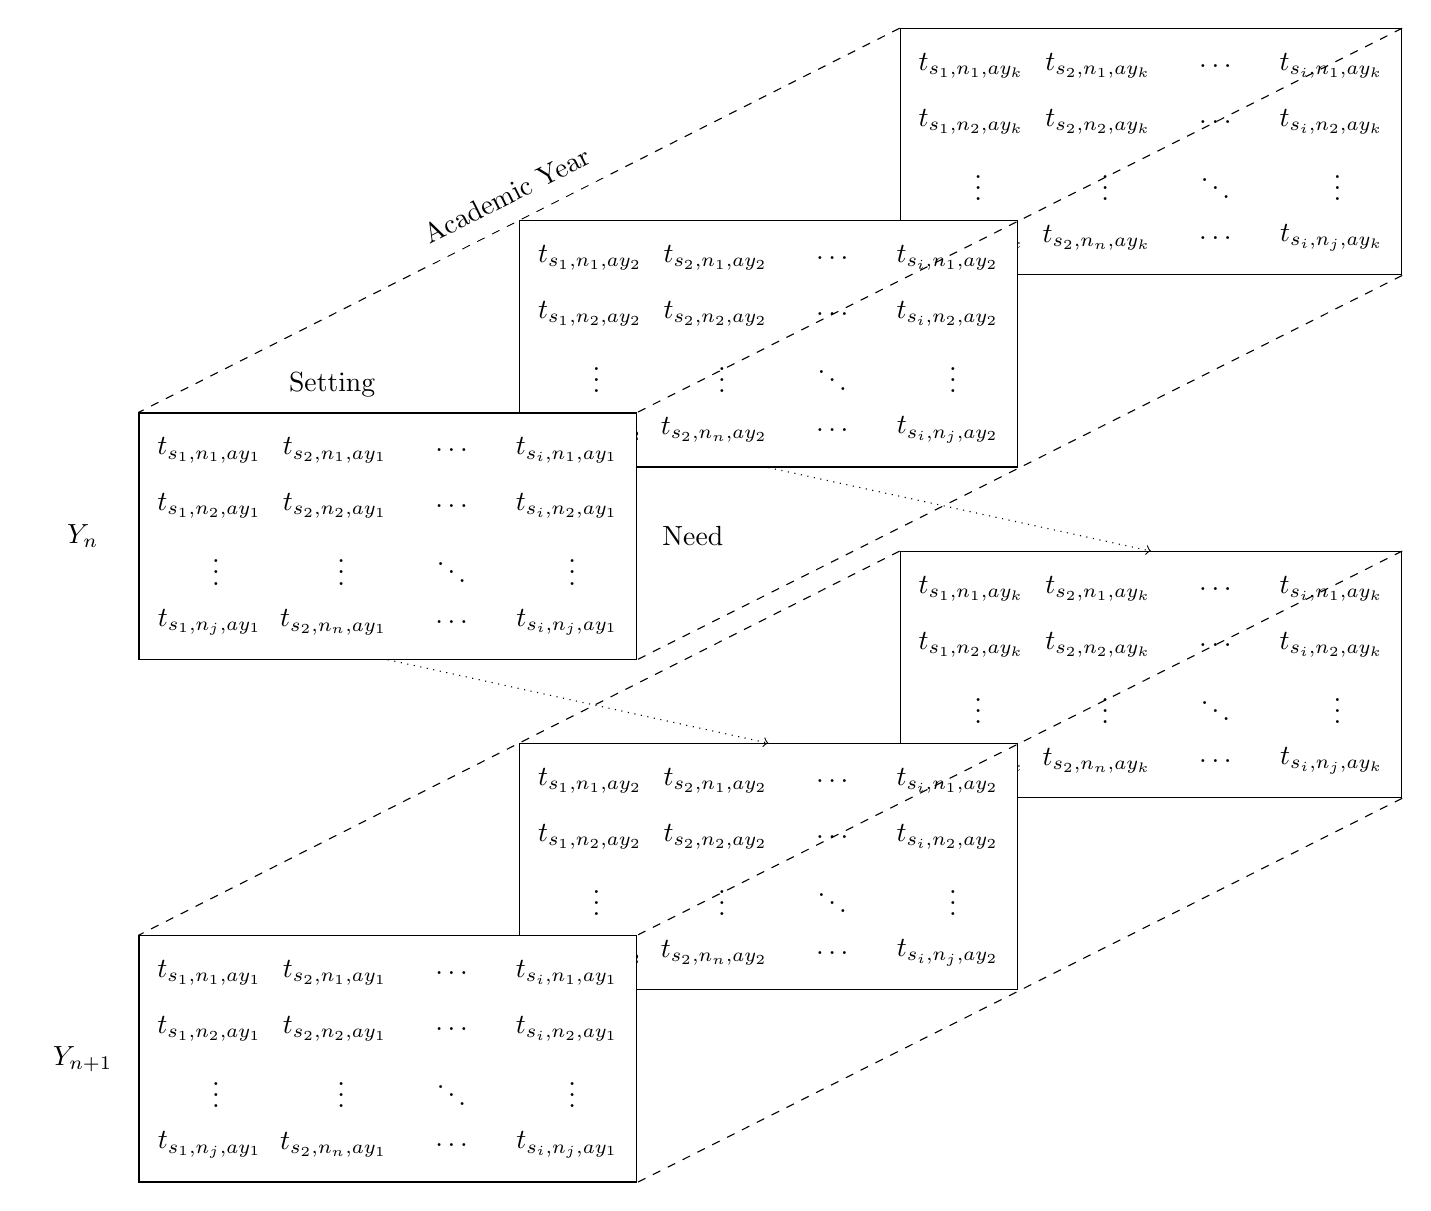
\begin{tikzpicture}[every node/.style={anchor=north
      east,fill=white,minimum width=1.4cm,minimum height=7mm}]

    \matrix (mA) [draw,matrix of math nodes]
    {
      t_{s_1,n_1,ay_k} & t_{s_2,n_1,ay_k} & \dots & t_{s_i,n_1,ay_k} \\
      t_{s_1,n_2,ay_k} & t_{s_2,n_2,ay_k} & \dots & t_{s_i,n_2,ay_k} \\
      \vdots & \vdots & \ddots & \vdots \\
      t_{s_1,n_j,ay_k} & t_{s_2,n_n,ay_k} & \dots & t_{s_i,n_j,ay_k} \\
    };

    \matrix (mB) [draw,matrix of math nodes] at ($(mA.south west)+(1.5,0.7)$)
    {
      t_{s_1,n_1,ay_2} & t_{s_2,n_1,ay_2} & \dots & t_{s_i,n_1,ay_2} \\
      t_{s_1,n_2,ay_2} & t_{s_2,n_2,ay_2} & \dots & t_{s_i,n_2,ay_2} \\
      \vdots & \vdots & \ddots & \vdots \\
      t_{s_1,n_j,ay_2} & t_{s_2,n_n,ay_2} & \dots & t_{s_i,n_j,ay_2} \\
    };

    \matrix (mC) [draw,matrix of math nodes] at ($(mB.south west)+(1.5,0.7)$)
    {
      t_{s_1,n_1,ay_1} & t_{s_2,n_1,ay_1} & \dots & t_{s_i,n_1,ay_1} \\
      t_{s_1,n_2,ay_1} & t_{s_2,n_2,ay_1} & \dots & t_{s_i,n_2,ay_1} \\
      \vdots & \vdots & \ddots & \vdots \\
      t_{s_1,n_j,ay_1} & t_{s_2,n_n,ay_1} & \dots & t_{s_i,n_j,ay_1} \\
    };

    \draw[dashed](mA.north east)--(mC.north east);
    \draw[dashed](mA.north west)-- node[sloped,above] {Academic Year} (mC.north west);
    \draw[dashed](mA.south east)--(mC.south east);

    \node [above left] at (mC.north) {Setting};
    \node [right] at (mC.east) {Need};
    \node [left] at (mC.west) {$Y_n$};

    \matrix (mD) [draw,matrix of math nodes] at ($(mA.south east)+(0,-3.5)$)
    {
      t_{s_1,n_1,ay_k} & t_{s_2,n_1,ay_k} & \dots & t_{s_i,n_1,ay_k} \\
      t_{s_1,n_2,ay_k} & t_{s_2,n_2,ay_k} & \dots & t_{s_i,n_2,ay_k} \\
      \vdots & \vdots & \ddots & \vdots \\
      t_{s_1,n_j,ay_k} & t_{s_2,n_n,ay_k} & \dots & t_{s_i,n_j,ay_k} \\
    };

    \matrix (mE) [draw,matrix of math nodes] at ($(mB.south east)+(0,-3.5)$)
    {
      t_{s_1,n_1,ay_2} & t_{s_2,n_1,ay_2} & \dots & t_{s_i,n_1,ay_2} \\
      t_{s_1,n_2,ay_2} & t_{s_2,n_2,ay_2} & \dots & t_{s_i,n_2,ay_2} \\
      \vdots & \vdots & \ddots & \vdots \\
      t_{s_1,n_j,ay_2} & t_{s_2,n_n,ay_2} & \dots & t_{s_i,n_j,ay_2} \\
    };

    \matrix (mF) [draw,matrix of math nodes] at ($(mC.south east) + (0,-3.5)$)
    {
      t_{s_1,n_1,ay_1} & t_{s_2,n_1,ay_1} & \dots & t_{s_i,n_1,ay_1} \\
      t_{s_1,n_2,ay_1} & t_{s_2,n_2,ay_1} & \dots & t_{s_i,n_2,ay_1} \\
      \vdots & \vdots & \ddots & \vdots \\
      t_{s_1,n_j,ay_1} & t_{s_2,n_n,ay_1} & \dots & t_{s_i,n_j,ay_1} \\
    };

    \draw[dashed](mD.north east)--(mF.north east);
    \draw[dashed](mD.north west)--(mF.north west);
    \draw[dashed](mD.south east)--(mF.south east);

    \draw[dotted,->](mC.south)--(mE.north);
    \draw[dotted,->](mB.south)--(mD.north);

    \node [left] at (mF.west) {$Y_{n+1}$};
  \end{tikzpicture}
  \caption{System state from one calendar year to the next\label{state}
  }
\end{figure}

The initial system state, is constructed from the historic data
provided by the client (we simply count the number of pupils that, for
example, match $(s_1,n_1,ay_1)$, in a calendar year).

In Fig.\ref{state} you can think of $Y_n$ as a 3-dimensional matrix of
population values, representing the pupil populations of the set of
unique entities in year n.  $Y_{n+1}$ is the next system state for the
following calendar year.

\section{SEND Model's Population Prediction Algorithm}

The crux of the SEND Model's prediction algorithm is to take us from
$Y_n$ to $Y_{n+1}$ in Fig.\ref{state}. From \ref{summary} we know in
addition to our starting state we also use external pupil population
predictions and historic data to generate probability distributions.
Thus:

$Y_{n+1} = T(Y_n,P_{ext}, H)$

$Y_n$ represents calendar year $n$'s system state.

$P_{ext}$ represents the external pupil population predictions.

$H$ represents the historic data.

$T$ is the function that calculates the next years system state.

To simplify our scope when trying to understand $T$ let us consider
first a single entity only.  How will that entity's population
$t_{s_x,n_y,ay_z}$ be used to predict the following years?  How are
$P_{ext}$ and $H$ used to support this?

In all the following sections except where noted it is assumed that
the underlying processes governing leavers, joiners, and movers are
independent and identically distributed meaning that we can combine
historic calendar years data, $H$, as one.

\subsection{Movers, Remainers, Leavers and Joiners}

First we must understand the model's concepts of movers($m$),
remainers($r$), leavers($l$), and joiners($j$).

Let $m_{s_x,n_y,ay_z}$ be defined as all the pupils that move
\textbf{into} a particular entity from another entity that has a
different need or setting.  We deliberately exclude academic year from
the definition as if only this changes then we consider the move to be
part of the remainers.

Let $r_{s_x,n_y,ay_z}$ be defined as all the pupils that move out of a
particular entity and into another entity with the same need and
setting but different academic year.

Let $l_{s_x,n_y,ay_z}$ be defined as all the pupils that
\textbf{leave} a particular entity and out of the SEND programme
completely.

Let $j_{s_x,n_y,ay_z}$ be defined as all the pupils that join
\textbf{into} a particular entity from the outside populace.

So $T(Y_n,P_{ext}, H)_{s_x,n_y,ay_z} = m_{s_x,n_y,ay_z} + r_{s_x,n_y,ay_z} -
l_{s_x,n_y,ay_z} + j_{s_x,n_y,ay_z} $

Reading this equation aloud makes obvious intuitive sense.  The
question now becomes how do we calculate each of the components of
this function?

\subsection{Leavers}

From our historic data we can work out the percentages over the
calendar years of how many pupils leave a particular entity,
$(s_1,n_1,ay_1)$.  Averaging this sets our expectation e.g. for
$(s_1,n_1,ay_1)$ we may expect $40\%$ of the population to leave.

For the purposes of our simulation we do not want every run to have
exactly $40\%$ of the population leave but rather have some variance
in the size.  How these variances in the population propagate through
the simulation lets us see confidence bounds when we come to
aggregate the results of many runs of the model.

A first pass at introducing variance is to use the binomial
distribution to alter the population that leaves per run.

Continuing our example given $t_{s_1,n_1,ay_1} = 100$ and an
expectation of $40\%$ then a sample of ten values looks like so:

\begin{lstlisting}
(sample 10 (binomial {:n 100 :p 0.4}))
(46 42 31 45 43 44 48 41 41 40)
\end{lstlisting}

We can further refine the introduction of variance by noting that the
expectation of the percentage of leavers is stronger or weaker (more
or less confident in) depending on the amount of data in $H$ we have.
Intuitively if we have lots of observations around the number of
leavers then we can be much more confident in our expected value.  If
we have very few observations then we are much less confident its true
underlying value.

The beta distribution can be used to express the variance in our
expected leaver percentage (40\% or 0.4 in the above example).  The
parameters for the distribution $\alpha$, $\beta$ are simply the
observed leavers and non-leavers respectively.  Drawing from the beta
distribution is equivalent to working out the percentage expectation
(obviously slightly changed as it's purpose is to introduce variance
in this value).  For low values of observations there will be a wide
range in the values of the expected leavers and for high values of
observations there will be a much narrower range of expected values.

If we use the results of the Beta distribution as the probability
parameter of the Binomial distribution (composition) we form what's
called a hierarchical model.  This chaining of distributions increases
the size of variance in our model runs.

Thus we can write:

\begin{equation*}
l_{s_x,n_y,ay_z} = \text{Binomial}(t_{s_x,n_y,ay_z},
\text{Beta}(\alpha^l_{s_x,n_y,ay_z}, \beta^l_{s_x,n_y,ay_z}))
\end{equation*}

where $\alpha^l_{s_x,n_y,ay_z}$ represents the count of leavers over
all historic calendar years for the entity $({s_x,n_y,ay_z})$.
Similarly $\beta^l_{s_x,n_y,ay_z}$ represents the count of all non
leavers for the same entity over all historic calendar years.
$(t_{s_x,n_y,ay_z}$ represents the population of the entity.

To recap, the beta distribution using the historical leavers and
non-leavers is drawn from once per calculation to find the probability
someone leaves.  Then using this probability and the population of the
entity we use the binomial distribution to draw a value for pupils
that leave.  This is a common pattern throughout the model and is
important to understand well.

\subsection{Joiners}

The calculation for working out an entity's joiners is split into two
parts: first the expected rate of joiners is calculated per academic
year, then this additional population is assigned a need and setting.

The sum of the joiners for a single academic year over all historic
calendar years is first calculated.  As for leavers we wish calculate
the probability of joining SEND - we know that if we have the
non-leavers we can use the beta distribution to draw a probability
value of joining.

We work out the number of non-joiners by taking the joiners away from
the predicted number of pupils for an AY across the entire school
system: both send and non-send.  This external data source, $P_{ext}$,
might, for example, be the ONS data.  Typically $P_{ext}$ is only
available at an AY level.  Our desire to use it means that we can't
work at the normal ${s_x,n_y,ay_z}$ level - and explains why are
considering joiners over an entire academic year rather than an entity.

We once more use the binomial distribution to provide variance in
our population values once we have an expected probability from the
beta distribution.  Thus:

\begin{equation*}
j_{ay_z} = \text{Binomial}(p_{ay},
\text{Beta}(\frac{\alpha^j_{ay_z}}{cy_{obs}},\frac{p^{H}_{ay} -\alpha^j_{ay_z}}{cy_{obs}})
\end{equation*}

where $\alpha^j_{ay_z}$ is the total joiners for $ay_z$ (from the
historic calendar years), $cy_{obs}$ is the number of observed
calendar years, $p_{ay_z}$ is the projected population from our
additional population source for $ay_z$, and $p^{H}_{ay}$ is the total
population count over the historic calendar years.

You may notice an oddity in this equation, in our code-base we divide
through the sum of the joiners and non-joiners by observed calendar
years.  This has the effect of increasing variance.  It is in direct
contrast to the other probability distribution calculations that
assume independent and identical distributions.  Why this is done is
in under-investigation.

The second part of the calculation is to distribute the new joiners to
appropriate needs and settings.  We count for each academic year
exactly how many joiners there are from non-SEND to each of the
need-settings.  The proportions of which tell us how to distribute the
joiners.  Note: this time we don't divide through by the academic
years.  Armed with these proportions we can calculate the expectation
as a percentage for each e.g $10\%$ to $(s_x,n_y,ay_z)$ and $90\%$ to
$(s_j,n_k,ay_l)$.

Again, rather then a direct calculation of the population to be
assigned to each entity we introduce variance by using the multinomial
distribution.  It performs exactly the same job as the binomial except
over multiple possible outcomes.

In a now familiar pattern, we also wish to introduce variance in the
actual percentages used to calculate the assignment.  Like before, we
want high confidence in values we have lots of observed data for and
low confidence for few observations.  The Dirichlet distribution does
this for multivariates in exactly the same way beta distribution does
for two.  We combine the two to produce another hierarchical model.

\begin{equation*}
\begin{split}
  \text{Multinomial} ( & j_{ay_{z}}, \\
  & \text{Dirichlet} (\alpha^{j}_{s_x,n_y,ay_z}, \dots,
  \alpha^{j''}_{s_{x'''},n_{y''},ay_{z''}}))
\end{split}
\end{equation*}

Here the $\alpha^{j}$s represent the total number of transitions from
$non\-SEND$ to ${s_x,n_y,ay_z}$.

The results of the multinomial function is however a vector of the
counts of the joiners for each of the possible entities.  Thus for any
particular entity of interest we need to take the appropriate index.

\begin{equation*}
  \begin{split}
    j_{s_x,n_y,ay_z} = \bigg[\text{Multinomial}( & j_{ay_z}, \\
    & \text{Dirichlet}(\alpha^{j}_{s_x,n_y,ay_z},\alpha^{j'}_{s_{x'},n_{y'},ay_{z'}}, \dots, \alpha^{j''}_{s_{x''},n_{y''},ay_{z''}}))\bigg]_{s_x,n_y,ay_z}
  \end{split}
\end{equation*}

We can write this out in full for single entity by expanding
$j_{ay_z}$.

\begin{equation*}
  \begin{split}
j_{s_x,n_y,ay_z} = \bigg[\text{Multinomial}( & \text{Binomial}(p_{ay_z},
\text{Beta}(\frac{\alpha^j_{ay_z}}{cy_{obs}},\frac{p^{H}_{ay} -\alpha^j_{ay_z}}{cy_{obs}}), \\
& \text{Dirichlet}(\alpha^{j}_{s_x,n_y,ay_z}, \dots
, \alpha^{j''}_{s_{x''},n_{y''},ay_{z''}}))\bigg]_{s_x,n_y,ay_z}
  \end{split}
\end{equation*}

Interestingly, we can immediately see that the number of joiners to an
entity is not directly related to that entity's population state,
rather its relation is to the projected population for an academic year
and the non-SEND to entity transitions in the observed data.

\subsection{Movers and Remainers}


The core form of the calculation for movers should be by now familiar.

\begin{equation*}
  \begin{split}
m^{out}_{s_x,n_y,ay_z} =
\text{Multinomial}( & \text{Binomial}(t_{s_x,n_y,ay_z} - l_{s_x,n_y,ay_z}, 
 \text{Beta}(\alpha^m_{s_x,n_y,ay_z},\beta^m_{s_x,n_y,ay_z})),
\\ &  \text{Dirichlet}(\alpha^{m'}_{s_x',n_y',ay_z'}, \dots,
\alpha^{m''}_{s_{x''},n_{y''},ay_{z''}}))
\end{split}
\end{equation*}

The superscript $out$ represents the fact this equation actually
provides a vector of the pupils that leave ${s_x,n_y,ay_z}$ not move
into it.  How we deal with that we'll come to later.

Like leavers the relationship is based on the current entity's
population count (not the academic year's population count).  However
it is slightly modified in that we take the previously calculated
leavers away for this entity (as we know they move to non-SEND).

The Beta params $\alpha^m$ and $\beta^m$ are the counts of the
transitions out-of-${s_x,n_y,ay_z}$-and-into-some-other-setting and the
transitions to-itself respectively.  Unlike joiners they are not
divided through by observed calendar years.

The Dirichlet params $\alpha^{m'}$'s are the counts from the observed
data of our entity ${s_x,n_y,ay_z}$ to the other entities it can move
to ${s_x',n_y',ay_z'}$ (represented by ever increasing dashes).  As
such the vector that is the result of the multinomial has no count of
any movers to our entity ${s_x,n_y,ay_z}$.  Instead we need to
calculate $m^{out}$ for every other entity and take from each
generated vector the index that represents the population that moves
to $m_{s_x,n_y,ay_z}$.  The sum of these is the total movers into our
entity.

\begin{equation*}
  \begin{split}
    m_{s_x,n_y,ay_z} = \sum_{j \neq x, k \neq y , l \neq z }\bigg[
        \text{Multinomial}( & \text{Binomial}(t_{s_j,n_k,ay_l} - l_{s_j,n_k,ay_l}, 
        \text{Beta}(\alpha^m_{s_j,n_k,ay_l},\beta^m_{s_j,n_k,ay_l})),
        \\ &  \text{Dirichlet}(\alpha^{m'}_{s_j',n_k',ay_l'}, \dots,
        \alpha^{m''}_{s_{j''},n_{k''},ay_{l''}}))\bigg]_{s_x,n_y,ay_z}
\end{split}
\end{equation*}

where $j$, $k$, $l$ belong to $S$, $N$, $AY$ respectively.

As we know that remainers for an entity move to an entity with the
same need setting but in the next academic year we just use the beta
binomial to calculate these.

\begin{equation*}
  \begin{split}
    r_{s_x,n_y,ay_z} = & t_{s_x,n_y,ay_z}
    - l_{s_x,n_y,ay_z} \\ & - \text{Binomial}(t_{s_x,n_y,ay_z} - l_{s_x,n_y,ay_z}, 
\text{Beta}(\alpha^m_{s_x,n_y,ay_z},\beta^m_{s_x,n_y,ay_z}))
\end{split}
\end{equation*}

For consistency of the model that Binomial component of the above
equation should be the same result as when it was used to calculate
the movers.

\subsection{The Full Algorithm}

Calculate next years $t$ for an entity given the current
years state, $Y_n$, predicted pupil population, $P_{ext}$, and
historic data $H$.

\begin{equation*}
  \begin{aligned}
    \begin{split}
      Y_{n+1, s_x,n_y,ay_z} & = T(Y_n,P_{ext}, H)_{s_x,n_y,ay_z} \\
      & = m_{s_x,n_y,ay_z} + r_{s_x,n_y,ay_z} -
l_{s_x,n_y,ay_z} + j_{s_x,n_y,ay_z}
\end{split}
\end{aligned}
\end{equation*}
Where

\begin{equation*}
\begin{aligned}
& \begin{split}
    m_{s_x,n_y,ay_z} = \sum_{j \neq x, k \neq y , l \neq z }\bigg[
        \text{Multinomial}( & \text{Binomial}(t_{s_j,n_k,ay_l} - l_{s_j,n_k,ay_l}, 
        \text{Beta}(\alpha^m_{s_j,n_k,ay_l},\beta^m_{s_j,n_k,ay_l})),
        \\ &  \text{Dirichlet}(\alpha^{m'}_{s_j',n_k',ay_l'}, \dots,
        \alpha^{m''}_{s_{j''},n_{k''},ay_{l''}}))\bigg]_{s_x,n_y,ay_z}
\end{split}\\ 
& \begin{split}
    r_{s_x,n_y,ay_z} = t_{s_x,n_y,ay_z}  - l_{s_x,n_y,ay_z} & - \text{Binomial}(t_{s_x,n_y,ay_z} - l_{s_x,n_y,ay_z}, 
    & \text{Beta}(\alpha^m_{s_x,n_y,ay_z},\beta^m_{s_x,n_y,ay_z})) 
  \end{split}\\
& \begin{split}
  l_{s_x,n_y,ay_z} =
  \text{Binomial}(t_{s_x,n_y,ay_z},\text{Beta}(\alpha^l_{s_x,n_y,ay_z},
  \beta^l_{s_x,n_y,ay_z}))
\end{split}\\
& \begin{split}
j_{s_x,n_y,ay_z} = \bigg[\text{Multinomial}( & \text{Binomial}(p_{ay_z},
\text{Beta}(\frac{\alpha^j_{ay_z}}{cy_{obs}},\frac{p^{H}_{ay} -\alpha^j_{ay_z}}{cy_{obs}}), \\
& \text{Dirichlet}(\alpha^{j}_{s_x,n_y,ay_z}, \dots
, \alpha^{j''}_{s_{x''},n_{y''},ay_{z''}}))\bigg]_{s_x,n_y,ay_z}
\end{split}\\
\end{aligned}
\end{equation*}

The $\alpha$ and $\beta$ parameters to the Beta and Dirichlet
distributions are calculated in advance from the historic data $H$.

The joiner calculation requires $P_{ext}$ to provide the data for the
general population.

The entire current state $Y_n$ is required to work out a single
entity's future population: this is because we use the entire AY
population in the joiner calculation and we need to sum all movers
into our entity from all the other entities.

\section{A Case Study}

We go through the calculation of an entity's next state (via the
leaver and joiner calculations) to show how the algorithm works and to
embed the meaning of the myriad of parameters.

Let us consider need $a$, setting $b$, in academic year $1$, the calendar
year of $2018$ - this entity at this time has a population of $100$.  The
algorithm will give us this entity's population for the next calendar
year 2019.

\begin{equation*}
  \begin{aligned}
    \begin{split}
      Y_{2019,s_a,n_b,ay_1} & = T(Y_{2018},P_{ext}, H)_{s_a,n_b,ay_1} \\
      &                    = m_{s_a,n_b,ay_1} + r_{s_a,n_b,ay_1} - l_{s_a,n_b,ay_1} + j_{s_a,n_b,ay_1}
\end{split}
\end{aligned}
\end{equation*}
and

$t_{s_a,n_b,ay_1} = 100$

First-off the leavers as it's the simplest:

\begin{equation*}
l_{s_a,n_b,ay_1} =
  \text{Binomial}(t_{s_a,n_b,ay_1},\text{Beta}(\alpha^l_{s_a,n_b,ay_1},
  \beta^l_{s_a,n_b,ay_1}))
\end{equation*}

Let's say we already know the expected rate of leavers is $40\%$ then

$t_{s_a,n_b,ay_1} \times 40\% = 100 \times 40 = 40$ pupils

We want variance in that so we use the binomial distribution to draw
some samples

\begin{equation*}
  \text{Binomial}(t_{s_a,n_b,ay_1}, 0.4) = \text{Binomial}(100, 0.4) = 38
\end{equation*}

Now we also want variance in the 0.4 value, so we use the Beta
distribution.  Assume that we have historic data, $H$, for the last 2
years that has 60 and 20 leavers, and 110 and 90 non-leavers
respectively.

\begin{equation*}
\text{Beta}(\alpha^l_{s_a,n_b,ay_1}, \beta^l_{s_a,n_b,ay_1}) =
\text{Beta}(60+20,110+90) = \text{Beta}(80,200) = 0.38
\end{equation*}

Combining this all together

\begin{equation*}
l_{s_a,n_b,ay_1} =
  \text{Binomial}(100,\text{Beta}(80,200)) = 43
\end{equation*}

Next let's look at joiners.

\begin{equation*}
  \begin{split}
j_{s_a,n_b,ay_1} = \bigg[\text{Multinomial}( & \text{Binomial}(p_{ay_1},
\text{Beta}(\frac{\alpha^j_{ay_1}}{cy_{obs}},\frac{p^{H}_{ay} -\alpha^j_{ay_1}}{cy_{obs}}), \\
& \text{Dirichlet}(\alpha^{j}_{s_x,n_y,ay_z}, \dots
, \alpha^{j''}_{s_{x''},n_{y''},ay_{z''}}))\bigg]_{s_a,n_b,ay_1}
  \end{split}
\end{equation*}

Let's assume our external population $p_{ay_1}$ is predicted to be a
1000 for $ay_1$ in 2019.

For our two years of historic data let's assume from $P_{ext}$ the
predicted populations are 900 and 1100.

Let's also say that the number of joiners in our historic data is 30
and 20 over all needs and settings for $ay_1$.

A first pass at expectation based on this data is:

$\frac{30+20}{900 + 1100} = 0.025$

As before we need would like some variance in this value, so we use
the beta distribution again.

\begin{equation*}
  \begin{split}
\text{Beta}(\frac{\alpha^j_{ay_1}}{cy_{obs}},\frac{p_{ay_1}
  -\alpha^j_{ay_1}}{cy_{obs}}) = \text{Beta}(\frac{20+30}{2},\frac{900
  + 1100 - 20 - 30}{2}) = \text{Beta}(25,975) = 0.02501
  \end{split}
\end{equation*}

note: ignore the division through by calendar years for now (it
doesn't effect expectation only the variance)

We once more use the binomial to get a varied value from the
population and the expectation.

$\text{Binomial}(p_{ay_1}, 0.02501) = \text{Binomial}(1000, 0.02501) = 25$

Armed with the fact we have 25 joiners for academic
year 1 in 2019 our equation reduces to:

\begin{equation*}
  \begin{split}
j_{s_a,n_b,ay_1} = \bigg[\text{Multinomial}(25, \text{Dirichlet}(\alpha^{j}_{s_a,n_b,ay_1}, \dots
, \alpha^{j''}_{s_{x''},n_{y''},ay_{1}}))\bigg]_{s_a,n_b,ay_1}
  \end{split}
\end{equation*}

This part deals with assigning those 25 pupils to specific entities.
Assuming our historic data for academic year one has one other valid
setting need c and setting d - what are the proportions of the
population between the two entities?

Let's say ab1 has populations of 20 and 40 over the two years and cd1
has populations of 60 an 80.  Then we can say 30\% of the population
is in ab1 and 70\% of the population is in cd1.

We can use these percentages to distribute the 25 joiners
appropriately.  As before we'd like to vary this and the Dirichlet
performs the same job as the Beta in this regard. So,

\begin{equation*}
  \begin{split}
\text{Dirichlet}(\alpha^{j}_{s_a,n_b,ay_1}, \dots,
\alpha^{j''}_{s_{x''},n_{y''},ay_{1}}) & =  \text{Dirichlet}(20 +
40_{s_a,n_b,ay_1}, 60 + 80_{s_c,n_d,ay_1}) \\
& = \text{Dirichlet}(60_{s_a,n_b,ay_1}, 140_{s_c,n_d,ay_1}) \\
& = [0.29_{s_a,n_b,ay_1}, 0.71_{s_c,n_d,ay_1}]
  \end{split}
\end{equation*}

Again rather than simply calculate the distribution based on these
percentages we introduce variance by using the multinomial to vary the
results (this plays the same role as the binomial from before).  Thus

\begin{equation*}
  \begin{split}
\text{Multinomial}(25, [0.29_{s_a,n_b,ay_1}, 0.71_{s_c,n_d,ay_1}]) = [
7_{s_a,n_b,ay_1}, 17_{s_c,n_d,ay_1}]
  \end{split}
\end{equation*}

The result is a vector and as we are calculating for only ${s_a,n_b,ay_1}$
the last thing we do is pull its index out (the square brackets in
the algorithm and its index represent that).  Thus we can now answer
the question of how many joiners will there be in the next calendar
year to ${s_a,n_b,ay_1}$.

$j_{s_a,n_b,ay_1} = 7$

These two walk-throughs should provide enough to understand the
mechanism for the movers and remainers.

\section{Other Things To Do}

\begin{itemize}
\item Priors section for leavers, joiners, movers
\item Scenarios
\item Valid state implications
\item The real simulation tick mechanism
\end{itemize}

\begin{appendices}
\section{To MC or not to MC}
This appendix deals with why the SEND model is Markov Chain like but
not actually Markov Chain based.  Rather it is closer to event
simulation.

\subsection{Markov Chain}

This section and the next explain how the SEND model would look if it
were implemented using just Markov Chains.  If we understand this we
understand why we can say the SEND Model is ``Markov like''.

The initial state of our Markov Chain, $Y_0$, is constructed from the
historic data provided by the client (we simply count the number of
pupils that, for example, match $(s_1,n_1,ay_1)$.

You can think of $Y_n$ as a 3-dimensional matrix of population values,
representing the pupil populations of the set of unique entities in
year n.

In Fig.\ref{state} $Y_{n+1}$ is the next state of our Markov Chain.

How we transition from $Y_{n}$ to $Y_{n+1}$ is the subject of the next
section.  However, it's worth noting now that the dotted arrows on the
diagram represent how the $t$'s of one academic year transition into
the next academic year, in the following calendar year.

The complete state of the model is represented as $S = \{Y_0, \dots,
Y_n\}$ where $n$ is the number of years we run the simulation for.

\subsection{Markov Transition Matrix}

In mathematics a Markov Transition Matrix is formally a matrix
containing the probability of transitioning between Markov states.
Conceptually, for the SEND Model, it can be thought of as telling us
what percentages of $t_{s_x,n_y,ay_z}$ will move to each of the
allowed entities $t_{s_x,n_y,ay_z}$ can move to.  Sometimes this is
referred to as \textit{rates}.

By looking at the historic data we could work out the expectation of
each of our transitions and build this matrix.  We visualise what this
looks like in Fig.\ref{transition matrix}.
\begin{figure}[h!]
  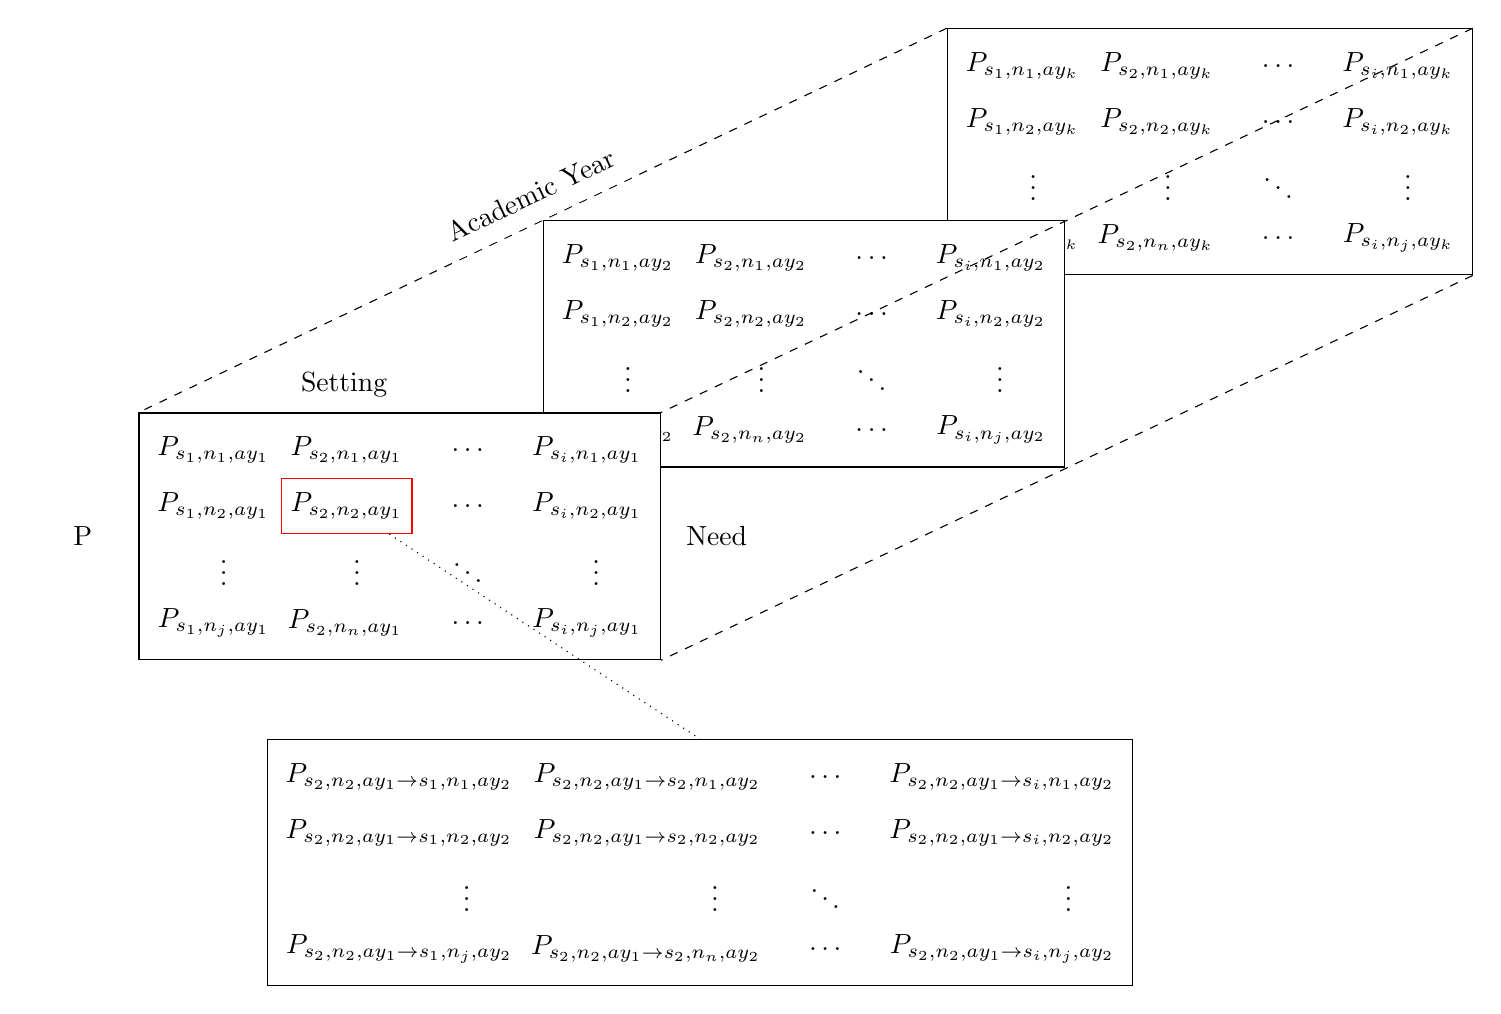
\begin{tikzpicture}[every node/.style={anchor=north east,fill=white,minimum width=1.4cm,minimum height=7mm}]

    \matrix (mA) [draw,matrix of math nodes]
    {
      P_{s_1,n_1,ay_k} & P_{s_2,n_1,ay_k} & \dots & P_{s_i,n_1,ay_k} \\
      P_{s_1,n_2,ay_k} & P_{s_2,n_2,ay_k} & \dots & P_{s_i,n_2,ay_k} \\
      \vdots & \vdots & \ddots & \vdots \\
      P_{s_1,n_j,ay_k} & P_{s_2,n_n,ay_k} & \dots & P_{s_i,n_j,ay_k} \\
    };

    \matrix (mB) [draw,matrix of math nodes] at ($(mA.south west)+(1.5,0.7)$)
    {
      P_{s_1,n_1,ay_2} & P_{s_2,n_1,ay_2} & \dots & P_{s_i,n_1,ay_2} \\
      P_{s_1,n_2,ay_2} & P_{s_2,n_2,ay_2} & \dots & P_{s_i,n_2,ay_2} \\
      \vdots & \vdots & \ddots & \vdots \\
      P_{s_1,n_j,ay_2} & P_{s_2,n_n,ay_2} & \dots & P_{s_i,n_j,ay_2} \\
    };

    \matrix (mC) [draw,matrix of math nodes] at ($(mB.south west)+(1.5,0.7)$)
    {
      P_{s_1,n_1,ay_1} & P_{s_2,n_1,ay_1} & \dots & P_{s_i,n_1,ay_1} \\
      P_{s_1,n_2,ay_1} & |[draw=red]|P_{s_2,n_2,ay_1} & \dots & P_{s_i,n_2,ay_1} \\
      \vdots & \vdots & \ddots & \vdots \\
      P_{s_1,n_j,ay_1} & P_{s_2,n_n,ay_1} & \dots & P_{s_i,n_j,ay_1} \\
    };

    \draw[dashed](mA.north east)--(mC.north east);
    \draw[dashed](mA.north west)-- node[sloped,above] {Academic Year} (mC.north west);
    \draw[dashed](mA.south east)--(mC.south east);

    \node [above left] at (mC.north) {Setting};
    \node [right] at (mC.east) {Need};
    \node [left] at (mC.west) {P};

    \matrix (mD) [draw,matrix of math nodes] at ($(mC.south east)+(6,-1)$)
    {
      P_{s_2,n_2,ay_1 \rightarrow s_1,n_1,ay_2} & P_{s_2,n_2,ay_1 \rightarrow s_2,n_1,ay_2} & \dots & P_{s_2,n_2,ay_1 \rightarrow s_i,n_1,ay_2} \\
      P_{s_2,n_2,ay_1 \rightarrow s_1,n_2,ay_2} & P_{s_2,n_2,ay_1 \rightarrow s_2,n_2,ay_2} & \dots & P_{s_2,n_2,ay_1 \rightarrow s_i,n_2,ay_2} \\
      \vdots & \vdots & \ddots & \vdots \\
      P_{s_2,n_2,ay_1 \rightarrow s_1,n_j,ay_2} & P_{s_2,n_2,ay_1 \rightarrow s_2,n_n,ay_2} & \dots & P_{s_2,n_2,ay_1 \rightarrow s_i,n_j,ay_2} \\
    };

    \draw[dotted](mC-2-2)--(mD.north);
  \end{tikzpicture}
  \caption{Markov Transition Matrix (many nested probability
    matrices)\label{transition matrix}
  }
\end{figure}

In the Fig.\ref{transition matrix} every $P_{s_i,n_j,ak_1}$ is a
probability matrix that represents the probabilities of transitioning
to any other state in the next academic year (see the diagram's
cut-out for an example.)

Armed with $P$, this rather complicated Markov Transition Matrix, we can
apply it to the initial state

$Y_1 = Y_0 \cdot P$

In fact at this point as $P$ is time independent we can work the
populations in year $n$ by

$Y_n = Y_0 \cdot P^n$

Of note is that this equation requires no tracking of $t$'s we can
simply use the above formula to work out $Y_n$. BUT we don't do this!
Why?

\subsection{SEND is not MC}

The SEND model actually sides step the creation of a Markov Transition
Matrix and takes an algorithmic approach to calculating $Y_{n+1}$'s
population.

This is done as some of the data is perhaps too sparse, but also the
algorithmic approach allows us to introduce priors and scenarios
rather more easily than modifying $P$ directly.

Further, we also use more than the just the initial state, in our
algorithmic predictions.  The model incorporates external population
data for each predicted calendar year.

As we will come to see the algorithmic approach to working out the
$t$'s in $Y_n$ introduces stochastic processes. Thus we introduce the
need to use Monte Carlo methods to ensure confidence in our
calculations.

The model can be thought of as a simulation with a simulation clock
that ticks once a calendar year. On clock tick all the entities have
their new population calculated: based on their existing state,
pre-calculated historic probability distributions and projected
population.
\end{appendices}

\begin{thebibliography}{9}

\bibitem{sma4}
  Averill M. Law,
  \textit{Simulation Modelling and Analysis},
  Addison Wesley, Massachusetts,
  4th edition,
  2007.

\end{thebibliography}
\end{document}


%%% Local Variables:
%%% mode: latex
%%% TeX-master: t
%%% End:
